\documentclass[journal,12pt,twocolumn]{IEEEtran}

\usepackage{setspace}
\usepackage{gensymb}

\singlespacing


\usepackage[cmex10]{amsmath}

\usepackage{amsthm}

\usepackage{mathrsfs}
\usepackage{txfonts}
\usepackage{stfloats}
\usepackage{bm}
\usepackage{cite}
\usepackage{cases}
\usepackage{subfig}

\usepackage{longtable}
\usepackage{multirow}

\usepackage{enumitem}
\usepackage{mathtools}
\usepackage{steinmetz}
\usepackage{tikz}
\usepackage{circuitikz}
\usepackage{verbatim}
\usepackage{tfrupee}
\usepackage[breaklinks=true]{hyperref}
\usepackage{graphicx}
\usepackage{tkz-euclide}
\usepackage{float}

\usetikzlibrary{calc,math}
\usepackage{listings}
    \usepackage{color}                                            %%
    \usepackage{array}                                            %%
    \usepackage{longtable}                                        %%
    \usepackage{calc}                                             %%
    \usepackage{multirow}                                         %%
    \usepackage{hhline}                                           %%
    \usepackage{ifthen}                                           %%
    \usepackage{lscape}     
\usepackage{multicol}
\usepackage{chngcntr}

\DeclareMathOperator*{\Res}{Res}

\renewcommand\thesection{\arabic{section}}
\renewcommand\thesubsection{\thesection.\arabic{subsection}}
\renewcommand\thesubsubsection{\thesubsection.\arabic{subsubsection}}

\renewcommand\thesectiondis{\arabic{section}}
\renewcommand\thesubsectiondis{\thesectiondis.\arabic{subsection}}
\renewcommand\thesubsubsectiondis{\thesubsectiondis.\arabic{subsubsection}}


\hyphenation{op-tical net-works semi-conduc-tor}
\def\inputGnumericTable{}                                 %%

\lstset{
%language=C,
frame=single, 
breaklines=true,
columns=fullflexible
}
\begin{document}


\newtheorem{theorem}{Theorem}[section]
\newtheorem{problem}{Problem}
\newtheorem{proposition}{Proposition}[section]
\newtheorem{lemma}{Lemma}[section]
\newtheorem{corollary}[theorem]{Corollary}
\newtheorem{example}{Example}[section]
\newtheorem{definition}[problem]{Definition}

\newcommand{\BEQA}{\begin{eqnarray}}
\newcommand{\EEQA}{\end{eqnarray}}
\newcommand{\define}{\stackrel{\triangle}{=}}
\newcommand\hlight[1]{\tikz[overlay, remember picture,baseline=-\the\dimexpr\fontdimen22\textfont2\relax]\node[rectangle,fill=blue!50,rounded corners,fill opacity = 0.2,draw,thick,text opacity =1] {$#1$};}
\bibliographystyle{IEEEtran}
\providecommand{\mbf}{\mathbf}
\providecommand{\pr}[1]{\ensuremath{\Pr\left(#1\right)}}
\providecommand{\qfunc}[1]{\ensuremath{Q\left(#1\right)}}
\providecommand{\sbrak}[1]{\ensuremath{{}\left[#1\right]}}
\providecommand{\lsbrak}[1]{\ensuremath{{}\left[#1\right.}}
\providecommand{\rsbrak}[1]{\ensuremath{{}\left.#1\right]}}
\providecommand{\brak}[1]{\ensuremath{\left(#1\right)}}
\providecommand{\lbrak}[1]{\ensuremath{\left(#1\right.}}
\providecommand{\rbrak}[1]{\ensuremath{\left.#1\right)}}
\providecommand{\cbrak}[1]{\ensuremath{\left\{#1\right\}}}
\providecommand{\lcbrak}[1]{\ensuremath{\left\{#1\right.}}
\providecommand{\rcbrak}[1]{\ensuremath{\left.#1\right\}}}
\theoremstyle{remark}
\newtheorem{rem}{Remark}
\newcommand{\sgn}{\mathop{\mathrm{sgn}}}
\providecommand{\abs}[1]{\left\vert#1\right\vert}
\providecommand{\res}[1]{\Res\displaylimits_{#1}} 
\providecommand{\norm}[1]{\left\lVert#1\right\rVert}
%\providecommand{\norm}[1]{\lVert#1\rVert}
\providecommand{\mtx}[1]{\mathbf{#1}}
\providecommand{\mean}[1]{E\left[ #1 \right]}
\providecommand{\fourier}{\overset{\mathcal{F}}{ \rightleftharpoons}}
%\providecommand{\hilbert}{\overset{\mathcal{H}}{ \rightleftharpoons}}
\providecommand{\system}{\overset{\mathcal{H}}{ \longleftrightarrow}}
	%\newcommand{\solution}[2]{\textbf{Solution:}{#1}}
\newcommand{\solution}{\noindent \textbf{Solution: }}
\newcommand{\cosec}{\,\text{cosec}\,}
\providecommand{\dec}[2]{\ensuremath{\overset{#1}{\underset{#2}{\gtrless}}}}
\newcommand{\myvec}[1]{\ensuremath{\begin{pmatrix}#1\end{pmatrix}}}
\newcommand{\mydet}[1]{\ensuremath{\begin{vmatrix}#1\end{vmatrix}}}
\numberwithin{equation}{subsection}
\makeatletter
\@addtoreset{figure}{problem}
\makeatother
\let\StandardTheFigure\thefigure
\let\vec\mathbf
\renewcommand{\thefigure}{\theproblem}
\def\putbox#1#2#3{\makebox[0in][l]{\makebox[#1][l]{}\raisebox{\baselineskip}[0in][0in]{\raisebox{#2}[0in][0in]{#3}}}}
     \def\rightbox#1{\makebox[0in][r]{#1}}
     \def\centbox#1{\makebox[0in]{#1}}
     \def\topbox#1{\raisebox{-\baselineskip}[0in][0in]{#1}}
     \def\midbox#1{\raisebox{-0.5\baselineskip}[0in][0in]{#1}}
\vspace{3cm}
\title{Challenge Problem 5}
\author{K.A. Raja Babu}
\maketitle
\newpage
\bigskip
\renewcommand{\thefigure}{\theenumi}
\renewcommand{\thetable}{\theenumi}
Download all python codes from 
\begin{lstlisting}
https://github.com/ka-raja-babu/Matrix-Theory/tree/main/ChallengeProblem5/Codes
\end{lstlisting}
%
and latex-tikz codes from 
%
\begin{lstlisting}
https://github.com/ka-raja-babu/Matrix-Theory/tree/main/ChallengeProblem5
\end{lstlisting}
%
\section{Challenge Question 5}

Express the axis of a parabola in terms of $\vec{V},\vec{u},f$ in general .

\section{Solution}

\begin{lemma}
Axis of any conic is given by
\begin{align}
    \boxed{\frac{\vec{e_2}^T\brak{\vec{x}-\vec{c}}}{{\vec{e_2}^T\vec{p}}} = \frac{\vec{e_1}^T\brak{\vec{x}-\vec{c}}}{{\vec{e_1}^T\vec{p}}}}
\end{align}
where,$\vec{c}$ is the vertex of conic and $\vec{p}$ is the eigen vector of $\vec{V}$ having smaller eigen value.
\end{lemma}

\begin{proof}
The general equation of a conic is
\begin{align}
  ax^2+2bxy+cy^2+2dx+2ey+f=0
\end{align}

which can be written in matrix form as
\begin{align}
    \vec{x}^T\vec{V}\vec{x} + 2\vec{u}^T\vec{x} + f =0
\end{align}

where,
\begin{align}
    \vec{V} &=\myvec{a & b \\ b& c}
    \\
    \vec{u} &= \myvec{d & e}
\end{align}

Let the vertex be
\begin{align}
    \vec{c} &= \myvec{x_c \\ y_c}
\end{align}

and,the origin be
\begin{align}
    \vec{O} &= \myvec{0 \\ 0}
\end{align}

and,the eigen vector of $\vec{V}$ having smaller eigen value be
\begin{align}
    \vec{p} &= \myvec{p_1 \\ p_2}
\end{align}

Now,according to the principal axis theorem,
\begin{enumerate}
    \item Each eigen vector of $\vec{V}$ is parallel to either major axis or minor axis.
    \item Eigen vectors of $\vec{V}$ are orthogonal to each other.
    \item Principal axes pass through the vertex $\vec{c}$ .
\end{enumerate}

Now,direction vector of eigen vector $\vec{p}$ is 
\begin{align}
    \vec{m_1} &= \vec{p}-\vec{O} \\
    \implies \vec{m_1} &= \myvec{p_1 \\ p_2} \\
    \implies \vec{m_1} &= p_1\myvec{1 \\ \frac{p_2}{p_1}} \\
    \implies \vec{m_1} &= \myvec{1 \\ \frac{p_2}{p_1}} \quad \brak{\because k\vec{m} \equiv \vec{m}} \\
    \implies \vec{m_1} &= \myvec{1 \\ \frac{\vec{e_2}^T\vec{p}}{\vec{e_1}^T\vec{p}}}
\end{align}

and,direction vector of axis is
\begin{align}
    \vec{m_2} &= \vec{x}-\vec{c}
    \\
    \implies \vec{m_2} &= \myvec{x-x_c \\ y-y_c} \\
    \implies \vec{m_2} &= \brak{x-x_c}\myvec{1 \\ \frac{y-y_c}{x-x_c}} \\
    \implies \vec{m_2} &= \myvec{1 \\ \frac{y-y_c}{x-x_c}}  \quad \brak{\because k\vec{m} \equiv \vec{m}} \\
    \implies \vec{m_2} &= \myvec{1 \\ \frac{\vec{e_2}^T\brak{\vec{x}-\vec{c}}}{\vec{e_1}^T\brak{\vec{x}-\vec{c}}}}
\end{align}
$\because$ Eigen vector is parallel to axis. \\
$\therefore$ Axis is given by
\begin{align}
    \vec{m_1} &= \vec{m_2} \\
    \implies \myvec{1 \\ \frac{\vec{e_2}^T\vec{p}}{\vec{e_1}^T\vec{p}}} &= \myvec{1 \\ \frac{\vec{e_2}^T\brak{\vec{x}-\vec{c}}}{\vec{e_1}^T\brak{\vec{x}-\vec{c}}}} \\ 
    \implies \frac{\vec{e_2}^T\vec{p}}{\vec{e_1}^T\vec{p}} &= \frac{\vec{e_2}^T\brak{\vec{x}-\vec{c}}}{\vec{e_1}^T\brak{\vec{x}-\vec{c}}} \\
    \implies \frac{\vec{e_2}^T\brak{\vec{x}-\vec{c}}}{{\vec{e_2}^T\vec{p}}} &= \frac{\vec{e_1}^T\brak{\vec{x}-\vec{c}}}{{\vec{e_1}^T\vec{p}}}
\end{align}

\end{proof}

\section{Examples}

\begin{enumerate}
    \item Parabola
    \begin{align}
    9x^2-24xy+16y^2-18x-101y+19 = 0
    \end{align}
    
    Here,
    \begin{align}
    \vec{V} &= \myvec{9 & -12 \\ -12 & 16} \\
    \vec{u} &= \myvec{-9 \\ \frac{-101}{2}} \\
    f &= 19
    \end{align}

    Now,
    \begin{align}
    \myvec{-39 & -73 \\ 9 & -12 \\ -12 & 16}\vec{c} &= \myvec{-19 \\ -21 \\ 28}
    \\
    \implies \vec{c} &= \myvec{\frac{-29}{25} \\ \frac{22}{25}}
    \end{align}
    
    So,
    \begin{align}
    \brak{\vec{x}-\vec{c}} &= \myvec{x+\frac{29}{25} \\ y-\frac{22}{25}}=\frac{1}{25}\myvec{25x+29 \\ 25y-22}
    \end{align}
    
    Now,
    \begin{align}
        \mydet{\vec{V}-\lambda\vec{I}} &= 0 \\
        \implies \mydet{9-\lambda & -12 \\ -12 & 16-\lambda} &= 0 \\
        \implies \lambda^2-25\lambda &= 0 \\
        \implies \lambda_1 =0,\lambda_2 &= 25
    \end{align}
    
    For $\lambda_1=0$,
    \begin{align}
        \vec{V}-\lambda_1\vec{I} &= \myvec{9 & -12 \\ -12 & 16} \\
        \implies \vec{V}-\lambda_1\vec{I} &= \myvec{1 & \frac{-4}{3} \\ 0 & 0} \\
        \implies \vec{p_1} &=\frac{3}{5}\myvec{\frac{4}{3} \\ 1}
    \end{align}
    
    Similarly for $\lambda_2=25$,
    \begin{align}
        \vec{p_2} &= \frac{4}{5}\myvec{\frac{-3}{4} \\ 1}
    \end{align}
    $\because \lambda_1<\lambda_2$ \\
    Hence,the axis using $\vec{p_1}$ is given by
    \begin{align}
        \frac{\vec{e_2}^T\brak{\vec{x}-\vec{c}}}{{\vec{e_2}^T\vec{p_1}}} &= \frac{\vec{e_1}^T\brak{\vec{x}-\vec{c}}}{{\vec{e_1}^T\vec{p_1}}}\\
        \implies \frac{y-\frac{22}{25}}{\frac{3}{5}} &= \frac{x+\frac{29}{25}}{\frac{4}{5}} \\
        \implies -75x+100y &= 175 \\
        \implies \boxed{\myvec{-3 & 4}\vec{x} = 7}
    \end{align}
    
    \numberwithin{figure}{section}
    \begin{figure}[!ht]
    \centering
    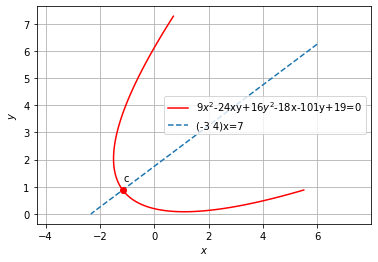
\includegraphics[width=\columnwidth]{ChallengeProblem5_1.png}
    \caption{9$x^2$-24xy+16$y^2$-18x-101y+19=0}
    \label{ex1}	
    \end{figure}
    
    \item Parabola
    \begin{align}
    y^2-4x+2y+4 = 0
    \end{align}
    
    Here,
    \begin{align}
    \vec{V} &= \myvec{0 & 0 \\ 0 & 1} \\
    \vec{u} &= \myvec{-2 \\ 1} \\
    f &= 4
    \end{align}

    Now,
    \begin{align}
    \myvec{-4 & 1 \\ 0 & 0 \\ 0 & 1}\vec{c} &= \myvec{-4 \\ 0 \\ -1}
    \\
    \implies \vec{c} &= \myvec{\frac{3}{4} \\ -1}
    \end{align}

    So,
    \begin{align}
    \brak{\vec{x}-\vec{c}} &= \myvec{x-\frac{3}{4} \\  y+1}
    \end{align}
    
    Now,
    \begin{align}
        \mydet{\vec{V}-\lambda\vec{I}} &= 0 \\
        \implies \mydet{-\lambda & 0 \\ 0 & 1-\lambda} &= 0 \\
        \implies \lambda_1 =0,\lambda_2 &= 1
    \end{align}
    
    For $\lambda_1=0$,
    \begin{align}
        \vec{V}-\lambda_1\vec{I} &= \myvec{0 & 0 \\ 0 & 1} \\
        \implies \vec{p_1} &= \myvec{1 \\ 0}
    \end{align}
    
    Similarly for $\lambda_2=1$,
    \begin{align}
        \vec{p_2} &=\myvec{0 \\ 1}
    \end{align}
    $\because \lambda_1<\lambda_2$ \\
    Hence,the axis using $\vec{p_1}$ is given by
    \begin{align}
        \frac{\vec{e_2}^T\brak{\vec{x}-\vec{c}}}{{\vec{e_2}^T\vec{p_1}}} &= \frac{\vec{e_1}^T\brak{\vec{x}-\vec{c}}}{{\vec{e_1}^T\vec{p_1}}}\\
        \implies \frac{y+1}{0} &= \frac{x-\frac{3}{4}}{1} \\
        \implies y+1 &= 0 \\
        \implies \boxed{\myvec{0 & -1}\vec{x} = -1}
    \end{align}
    
    \numberwithin{figure}{section}
    \begin{figure}[!ht]
    \centering
    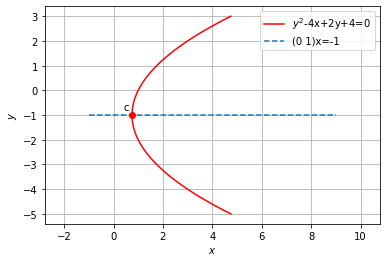
\includegraphics[width=\columnwidth]{ChallengeProblem5_2.png}
    \caption{$y^2$-4x+2y+4=0}
    \label{ex2}	
    \end{figure}
   
    \item Parabola
    \begin{align}
        y^2 &= 8x
        \\
        \implies y^2-8x &= 0
    \end{align}
    
    Here,
    \begin{align}
    \vec{V} &= \myvec{0 & 0 \\ 0 & 1} \\
    \vec{u} &= \myvec{-4 \\ 0} \\
    f &= 0
    \end{align}

    Now,
    \begin{align}
    \myvec{-8 & 1 \\ 0 & 0 \\ 0 & 1}\vec{c} &= \myvec{0 \\ 0 \\ 0}
    \\
    \implies \vec{c} &= \myvec{0 \\ 0}
    \end{align}
    
    So,
    \begin{align}
    \brak{\vec{x}-\vec{c}} &= \myvec{x \\ y}
    \end{align}
    
    Now,
    \begin{align}
        \mydet{\vec{V}-\lambda\vec{I}} &= 0 \\
        \implies \mydet{-\lambda & 0 \\ 0 & 1-\lambda} &= 0 \\
        \implies \lambda_1 =0,\lambda_2 &= 1
    \end{align}
    
    For $\lambda_1=0$,
    \begin{align}
        \vec{V}-\lambda_1\vec{I} &= \myvec{0 & 0 \\ 0 & 1} \\
        \implies \vec{p_1} &= \myvec{1 \\ 0}
    \end{align}
    
    Similarly for $\lambda_2=1$,
    \begin{align}
        \vec{p_2} &=\myvec{0 \\ 1}
    \end{align}
    $\because \lambda_1<\lambda_2$ \\
    Hence,the axis using $\vec{p_1}$ is given by
    \begin{align}
        \frac{\vec{e_2}^T\brak{\vec{x}-\vec{c}}}{{\vec{e_2}^T\vec{p_1}}} &= \frac{\vec{e_1}^T\brak{\vec{x}-\vec{c}}}{{\vec{e_1}^T\vec{p_1}}}\\
        \implies \frac{y}{0} &= \frac{x}{1} \\
        \implies y &= 0 \\
        \implies \boxed{\myvec{0 & 1}\vec{x} = 0}
    \end{align}

    \numberwithin{figure}{section}
    \begin{figure}[!ht]
    \centering
    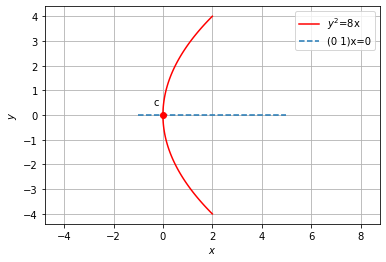
\includegraphics[width=\columnwidth]{ChallengeProblem5_3.png}
    \caption{$y^2$=8x}
    \label{ex3}	
    \end{figure}
    
    \item Ellipse
    \begin{align}
        x^2+xy+y^2 &= 100
    \end{align}
    
    Here,
    \begin{align}
    \vec{V} &= \myvec{1 & \frac{1}{2} \\ \frac{1}{2} & 1} \\
    \vec{u} &= \myvec{0 \\ 0} \\
    f &= -100
    \end{align}

    Now,
    \begin{align}
    \vec{c} &= \vec{V}^{-1}\vec{u}\\
    \implies \vec{c} &= \myvec{0 \\ 0}
    \end{align}

    So,
    \begin{align}
    \brak{\vec{x}-\vec{c}} &= \myvec{x \\ y}
    \end{align}
    
    Now,
    \begin{align}
        \mydet{\vec{V}-\lambda\vec{I}} &= 0 \\
        \implies \mydet{1-\lambda & \frac{1}{2} \\ \frac{1}{2} & 1-\lambda} &= 0 \\
        \implies \lambda^2-2\lambda+\frac{3}{4} &= 0 \\
        \implies \lambda_1 =\frac{1}{2},\lambda_2 &= \frac{3}{2}
    \end{align}
    
    For $\lambda_1=\frac{1}{2}$,
    \begin{align}
        \vec{V}-\lambda_1\vec{I} &= \myvec{\frac{1}{2} & \frac{1}{2} \\ \frac{1}{2} & \frac{1}{2}} \\
        \implies \vec{p_1} &= \frac{1}{\sqrt{2}}\myvec{-1 \\ 1}
    \end{align}
    
    Similarly for $\lambda_2=\frac{3}{2}$,
    \begin{align}
        \vec{p_2} &= \frac{1}{\sqrt{2}}\myvec{1 \\ 1}
    \end{align}
    $\because \lambda_1<\lambda_2$ \\
    Hence,the major axis using $\vec{p_1}$ is given by
    \begin{align}
        \frac{\vec{e_2}^T\brak{\vec{x}-\vec{c}}}{{\vec{e_2}^T\vec{p_1}}} &= \frac{\vec{e_1}^T\brak{\vec{x}-\vec{c}}}{{\vec{e_1}^T\vec{p_1}}}\\
        \implies \frac{y}{\frac{1}{\sqrt{2}}} &= \frac{x}{\frac{-1}{\sqrt{2}}} \\
        \implies y &= -x \\
        \implies \boxed{\myvec{1 & 1}\vec{x} = 0}
    \end{align}
    
    And,the minor axis using $\vec{p_2}$ is given by
    \begin{align}
        \frac{\vec{e_2}^T\brak{\vec{x}-\vec{c}}}{{\vec{e_2}^T\vec{p_2}}} &= \frac{\vec{e_1}^T\brak{\vec{x}-\vec{c}}}{{\vec{e_1}^T\vec{p_2}}}\\
        \implies \frac{y}{\frac{1}{\sqrt{2}}} &= \frac{x}{\frac{1}{\sqrt{2}}} \\
        \implies y &= x \\
        \implies \boxed{\myvec{-1 & 1}\vec{x} = 0}
    \end{align}
    
    \numberwithin{figure}{section}
    \begin{figure}[!ht]
    \centering
    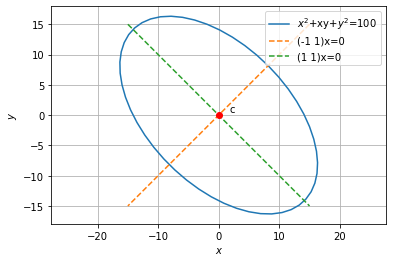
\includegraphics[width=\columnwidth]{ChallengeProblem5_4.png}
    \caption{$x^2$+xy+$y^2$=100}
    \label{ex4}	
    \end{figure}
    
    \item Hyperbola
    \begin{align}
        xy-3y+2 &= 0
    \end{align}
    
    Here,
    \begin{align}
    \vec{V} &= \frac{1}{2}\myvec{0 & 1 \\ 1 & 0} \\
    \vec{u} &= \frac{-3}{2}\myvec{0 \\ 1} \\
    f &= 2
    \end{align}

    Now,
    \begin{align}
    \vec{c} &= \vec{V}^{-1}\vec{u}\\
    \implies \vec{c} &= \myvec{3 \\ 0}
    \end{align}

    So,
    \begin{align}
    \brak{\vec{x}-\vec{c}} &= \myvec{x-3 \\ y}
    \end{align}

    Now,
    \begin{align}
        \mydet{\vec{V}-\lambda\vec{I}} &= 0 \\
        \implies \mydet{-\lambda & \frac{1}{2} \\ \frac{1}{2} & -\lambda} &= 0 \\
        \implies \lambda^2-\frac{1}{4} &= 0 \\
        \implies \lambda_1 =\frac{-1}{2},\lambda_2 &= \frac{1}{2}
    \end{align}
    
    For $\lambda_1=\frac{-1}{2}$,
    \begin{align}
        \vec{V}-\lambda_1\vec{I} &= \myvec{\frac{1}{2} & \frac{1}{2} \\ \frac{1}{2} & \frac{1}{2}} \\
        \implies \vec{p_1} &= \frac{1}{\sqrt{2}}\myvec{-1 \\ 1}
    \end{align}
    
    Similarly for $\lambda_2=\frac{1}{2}$,
    \begin{align}
        \vec{p_2} &= \frac{1}{\sqrt{2}}\myvec{1 \\ 1}
    \end{align}
    $\because \lambda_1<\lambda_2$ \\
    Hence,the major axis using $\vec{p_1}$ is given by
    \begin{align}
        \frac{\vec{e_2}^T\brak{\vec{x}-\vec{c}}}{{\vec{e_2}^T\vec{p_1}}} &= \frac{\vec{e_1}^T\brak{\vec{x}-\vec{c}}}{{\vec{e_1}^T\vec{p_1}}}\\
        \implies \frac{y}{\frac{1}{\sqrt{2}}} &= \frac{x-3}{\frac{-1}{\sqrt{2}}} \\
        \implies x+y &= 3\\
        \implies \boxed{\myvec{1 & 1}\vec{x} = 3}
    \end{align}
    
    And,the minor axis using $\vec{p_2}$ is given by
    \begin{align}
        \frac{\vec{e_2}^T\brak{\vec{x}-\vec{c}}}{{\vec{e_2}^T\vec{p_2}}} &= \frac{\vec{e_1}^T\brak{\vec{x}-\vec{c}}}{{\vec{e_1}^T\vec{p_2}}}\\
        \implies \frac{y}{\frac{1}{\sqrt{2}}} &= \frac{x-3}{\frac{1}{\sqrt{2}}} \\
        \implies -x+y &= 3 \\
        \implies \boxed{\myvec{-1 & 1}\vec{x} = 3}
    \end{align}
   
    \numberwithin{figure}{section}
    \begin{figure}[!ht]
    \centering
    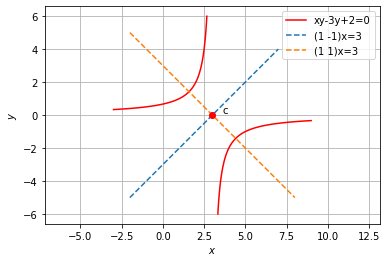
\includegraphics[width=\columnwidth]{ChallengeProblem5_5.png}
    \caption{xy-3y+2=0}
    \label{ex5}	
    \end{figure}
    
\end{enumerate}

\end{document}

